\documentclass[autodetect-engine,dvipdfmx-if-dvi,ja=standard]{bxjsarticle}

% 二段組にするとき
% \documentclass[twocolumn,autodetect-engine,dvipdfmx-if-dvi,ja=standard]{bxjsarticle}

\usepackage{graphicx}        %図を表示するのに必要
\usepackage{color}           %jpgなどを表示するのに必要
\usepackage{amsmath,amssymb} %数学記号を出すのに必要
\usepackage{setspace}
\usepackage{eclclass}
\usepackage{cases}
\usepackage{here}
\usepackage{fancyhdr}
\usepackage{ascmac}

% 文書全体のスタイルを設定(主に余白)
\setlength{\topmargin}{-0.3in}
\setlength{\oddsidemargin}{0pt}
\setlength{\evensidemargin}{0pt}
\setlength{\textheight}{44\baselineskip}

% 行頭の字下げをしない
\parindent = 0pt

% ヘッダとフッタの設定
\lhead{電気情報工学応用実験II}
\chead{}
\rhead{5E 20番 佐藤凌雅}
\lfoot{}
\cfoot{-\thepage-} % ページ数
\rfoot{}

% 式の番号を(senction_num.num)のようにする
\makeatletter
\@addtoreset{equation}{section}
\def\theequation{\thesection.\arabic{equation}}
\makeatother

% 画像の貼り付けを簡単にする
\newcommand{\pic}[2]
{
  \begin{figure}[H]
    \begin{center}
      \includegraphics[scale=#2]{#1}
    \end{center}
  \end{figure}
}

% 単位の記述を簡単にする
\newcommand{\unit}[1]
{
  \, [\mathrm{#1}]
}
\begin{document}
% \maketitle
\pagestyle{fancy}
\section{目的}
 立体導波管回路におけるマイクロ波の周波数測定法と定在波測定法の動作原理を理解する.

\section{予習}
マイクロ波回路用の空洞周波数計について構造や動作原理を調べよ.\\
 3ギガヘルツ以上のマイクロ波回路の周波数測定に用いられる装置.原理的には,寸法の定まった金属箱が,寸法に応じて定まる特定の波長のマイクロ波と共振する空胴共振器を利用して,波長の逆数としての周波数を測定する.\\

マイクロ波回路における,整合,反射係数,定在波,定在波比について調べよ.\\
・整合:信号源インピーダンスと負荷インピーダンスと伝送路の特性インピーダンスが等しくなった状態のこと\\
・反射係数:進行する波に対し反射して戻ってくる波の電圧振幅の割合のこと.\\
・定在波:周期,速さ,振幅が同一で逆方向に進行する波が重なると,波がその場で振動するように見える現象が生じる.この波のことを,定在波,あるいは定常波と呼ぶ.\\
・定在波比:定在波の最大の振幅と最小の振幅の比率.\\

\section{理論\label{riron}}
 高周波伝送には一般に同軸ケーブルが使用されるが,マイクロ波の周波数では表皮効果による損失が大きいため断面寸法比が2:1の方形導波管が使用される.\\
導波管による立体マイクロ波回路で金属製の様々な形状の回路素子があり,空洞による共振回路や金属板による減衰器,フィルタ,分岐や合成を行う部品等がある.\\
 高周波であるため分布定数回路として回路解析をする必要があり,特性インピーダンスの整合が取れない場合は反射はによる定在波が発生する.また,導波管での伝送は3次元的となり,通行の自由空間での電磁波の波長より長い管内波長をもつ.\\

導波管の遮断周波数 $f_c=c/\lambda c$\\
遮断波長$\lambda c = 2a$\\
管内波長 $\lambda_g = \dfrac{\lambda}{\sqrt{1-(\frac{\lambda}{\lambda_c})^2}}$\\
定在波比 $S=V_{max}/V_{min}=(1+\gamma)/(1-\gamma)$\\

\section{実験\label{jikken}}
\begin{enumerate}
    \item 測定器にクリスタルマウントをクリップで接続する.マイクロ波発振器専用電源のMODSELECTORをCWにし,投入後,電源電圧計が9Vであることを確認する.\\
    クリスタルマウント出力をuVメータで観測し,マイクロ波の存在を確認する.\\

    \item 空洞周波数計のつまみを回転させ,uVメーターの表示の最小点を探索せよ.ツマミの数値を読み周波数校正図から発信周波数を求めよ.\\

    \item 2.の測定周波数から自由空間のマイクロ波波長を計算で求める.次にノギスを用いて実験装置の導波管の長辺方向の内側寸法を計測し,遮断波長を求める。これらの測定値から管内波長を計算で求める.\\

    \item 定在波測定装置の探針を移動しながら探針のクリスタルマウント出力をuVメーターで測定し,グラフにプロットする.そのグラフから定在波の最小値間の距離Lを求める。\\

    \item 4.のVmaxとVminの値から,電圧定在波比を求め,さらに反射係数を計算で求めよ.\\
  \end{enumerate}

\newpage
\section{使用機器\label{kiki}}
・専用電源:SPC ELECTRONICS,TYPR 14T052,S/N R2780011,DATE 2013-7\\
・μVメータ:MODEL PM-18R,TOA Electronics Ltd.,SELIAL No.C96521D,昭和63年3月製造\\
・高調波除去用LPF:SPC ELECTRONICS,TYPE14T028,S/N R2780191,DATE 2013-7\\
・アイソレーター:SPC ELECTRONICS,TYPE 14T017A,S/N R2780161,DATE 2013-7\\
・可変抵抗減衰器:SPC ELECTRONICS,TYPE 14T003,S/N R2780021,DATE 2013-7\\
・空洞共振周波数計:SPC ELECTRONICS,TYPE 14T004,S/N R2780031,DATE 2013-7\\
・定在波測定器:SPC ELECTRONICS,TYPE 14T005,S/N R2780041,DATE 2013-7\\
・クリスタルマウント:KDR-IOSA,製造年月 1971-4 No.17416

\section{実験結果}
\subsection{実験\ref{jikken}.1}
 発振器の電源を投入したところ,電圧計は9Vを示した.また,クリスタルマウントの出力からマイクロ波の発生が確認できた.

\subsection{実験\ref{jikken}.2}
 クリスタルマウントの出力が最小となる点は2.95mmであった.周波数校正図から9365MHzであることが確認できた.

\subsection{実験\ref{jikken}.3}
 光速cは約300000000m/sである. また,測定された周波数fは9365000000Hzであった.$c/f$より自由空間のマイクロ波長は0.03203m(32.03mm)であることが分かった.\\
 次に,ノギスを用いて実験装置の導波管の長辺方向の内側寸法を計測したところ,23.05mmであることが分かった.\ref{riron}理論の導波管の遮断周波数の式より,遮断波長は46.10mmであった.以上の情報から管内波長は44.55mmであることが分かった.

\subsection{実験\ref{jikken}.4}
 クリスタルマウント出力を表1に示す.また,プロットしたグラフを図1に示す.\\
 また,最小値間の距離Lは22.5mmであった.この事実から管内波長は45.05mmであることが分かった.

\subsection{実験\ref{jikken}.5}
 前項の値から公式を用いて定在波比を計算したところ$S=12.63$であった.\\
 また,反射係数$\gamma$は$S=(1+\gamma)/(1-\gamma)$を$\gamma$について整理して,$\gamma=(S-1)/(1+S)$とし,これに代入して求めた.結果,$\gamma=0.8532$であった.

\newpage
\begin{table}[]
  \centering
  \caption{クリスタルマウント出力の距離特性}
  \begin{tabular}{|l|l||l|l|}
  \hline
  位置{[}mm{]} & 出力{[}mV{]} & 位置{[}mm{]} & 出力{[}mV{]} \\ \hline
  90& 9.1& 136& 11.0\\ \hline
  92& 12.0& 138& 12.1\\ \hline
  94& 12.7& 140& 12.0\\ \hline
  96& 11.2& 142& 10.0\\ \hline
  98& 9.0& 144& 7.3\\ \hline
  100& 5.8& 146& 4.3\\ \hline
  102& 2.8& 148& 1.8\\ \hline
  104& 1.2& 150& 0.9\\ \hline
  106& 1.3& 152& 2.0\\ \hline
  108& 3.3& 154& 4.4\\ \hline
  110& 6.4& 156& 7.4\\ \hline
  112& 9.5& 158& 10.5\\ \hline
  114& 12.0& 160& 12.2\\ \hline
  116& 12.9& 162& 12.5\\ \hline
  118& 12.0& 164& 11.0\\ \hline
  120& 10.0& 166& 8.6\\ \hline
  122& 7.0& 168& 5.4\\ \hline
  124& 3.7& 170& 2.5\\ \hline
  126& 1.5& 172& 1.1\\ \hline
  128& 1.1& 174& 1.6\\ \hline
  130& 2.6& 176& 3.8\\ \hline
  132& 5.3& 178& 7.1\\ \hline
  134& 8.4& 180& 10.0\\ \hline
  \end{tabular}
\end{table}

\newpage
\begin{landscape}
  \begin{figure}
    \centering
    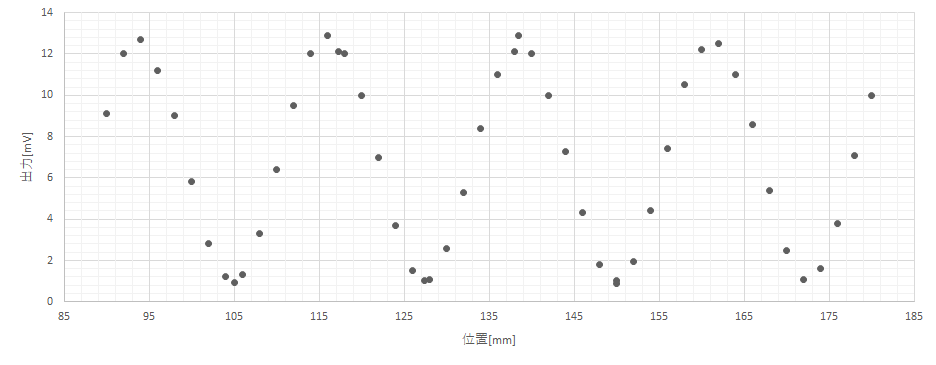
\includegraphics[width=25cm]{./data/data.png}
    \caption{クリスタルマウント出力の距離特性}
  \end{figure}
\end{landscape}

\newpage
\section{考察}
%  管内波長について実験\ref{jikken}.3と実験\ref{jikken}.4で求めた値を誤差も含めて比較検討せよ.\\
 実験\ref{jikken}.3で得た管内波長を真値として実験\ref{jikken}.4のデータとの誤差を求めると,0.454であった.この時の誤差率は1.019\%であった.\\
 この誤差率は小さいものと捉え,実験全般において大きなミスはなかったものと考える.\\
 1.019\% の誤差が発生した理由として考えられるのは,導波管の寸法測定誤差,uVの読み取り誤差などの測定に起因するものと,外部からの電磁的ノイズの影響などの環境的要因が考えられる.\\

%  定在波比や反射係数について,測定値と,理想的な伝搬状態での数値と比較して考察せよ.\\
 実験\ref{jikken}.5の結果から,定在波比と反射係数はそれぞれ$S=12.63$,$\gamma=0.8532$であった.\\
 定在波比は最大の振幅を持つ定在波の振幅と最小の振幅を持つ定在波の振幅の比を表している.すなわち,値の取りうる範囲は1から∞である.定在波比は1となる時,定在波がない,つまり反射波が存在しない理想的な伝送状態であると言える.今回の実験では,12.63であり,高い値となってしまったと考える.\\
 反射係数は反射波の電圧/進行波の電圧で定義され,反射波がどの程度存在するのかを表す指標である.この値は,0に近いほど良いとされる.今回の反射係数は0.85であり,定義上の最大値は1であることから考えるとこれもかなり高い値であった.\\
 以上の2つのパラメータから,伝送線路と負荷にインピーダンスの不連続 (不整合) が存在し,反射波が発生していたことがわかった.一般にこれらのパラメータを改善し,反射波の発生を抑えるために,インピーダンスマッチングなどが行われている.\\

\end{document}
